\section{Incorporating the body}

The passes so far have been preparatory ones, such that the main part of the algorithm can take place without problems.
This pass may seem out of place, but its purpose is to ensure that each code manipulation until the final result still
produces valid code, because this requirement is necessary later for resolving the method calls to the called methods
and finding the usages of the local variables using the infrastructure provided by Intellij IDEA.

The call stack is simulated in the method body by using a \code{stack} object. Whenever there is a call to the
containing method, a new frame object is pushed onto the \code{stack}. This is why after declaring the \code{stack}
object, the next statement in the body of the method is a \code{push} call, with the arguments equal to the formal
parameters. This frame represents the first method call from outside this method.

If the return type of the method is not \code{void}, the next statement in the method body is a declaration
statement of a local variable named \code{ret}, which is used to save the return value of the callee, to be used
later by the caller in a recursive call.

The next statement is a \code{while} statement which loops as long as the simulated call \code{stack} is not empty.
Because the body of the statement executes the code in the context of a current stack \code{frame},
the first statement in the \code{while} body is a declaration statement of a local variable named \code{frame},
initialized as the frame at the top of the call stack. After this statement, the original body of the method is
included here as a block statement.

If the return type of the method is not \code{void}, there is a final \code{return} statement in the method body
after the \code{while} statement, which returns the value of the \code{ret} local variable, which holds the
return value of the method after the control flow exits the \code{while} statement.

An example of this pass is provided in \labelindexref{Figure}{img:incorporate}.

\begin{figure}[htb]
    \makebox[\linewidth][c]{%
    \begin{subfigure}[b]{.6\textwidth}
        \centering
        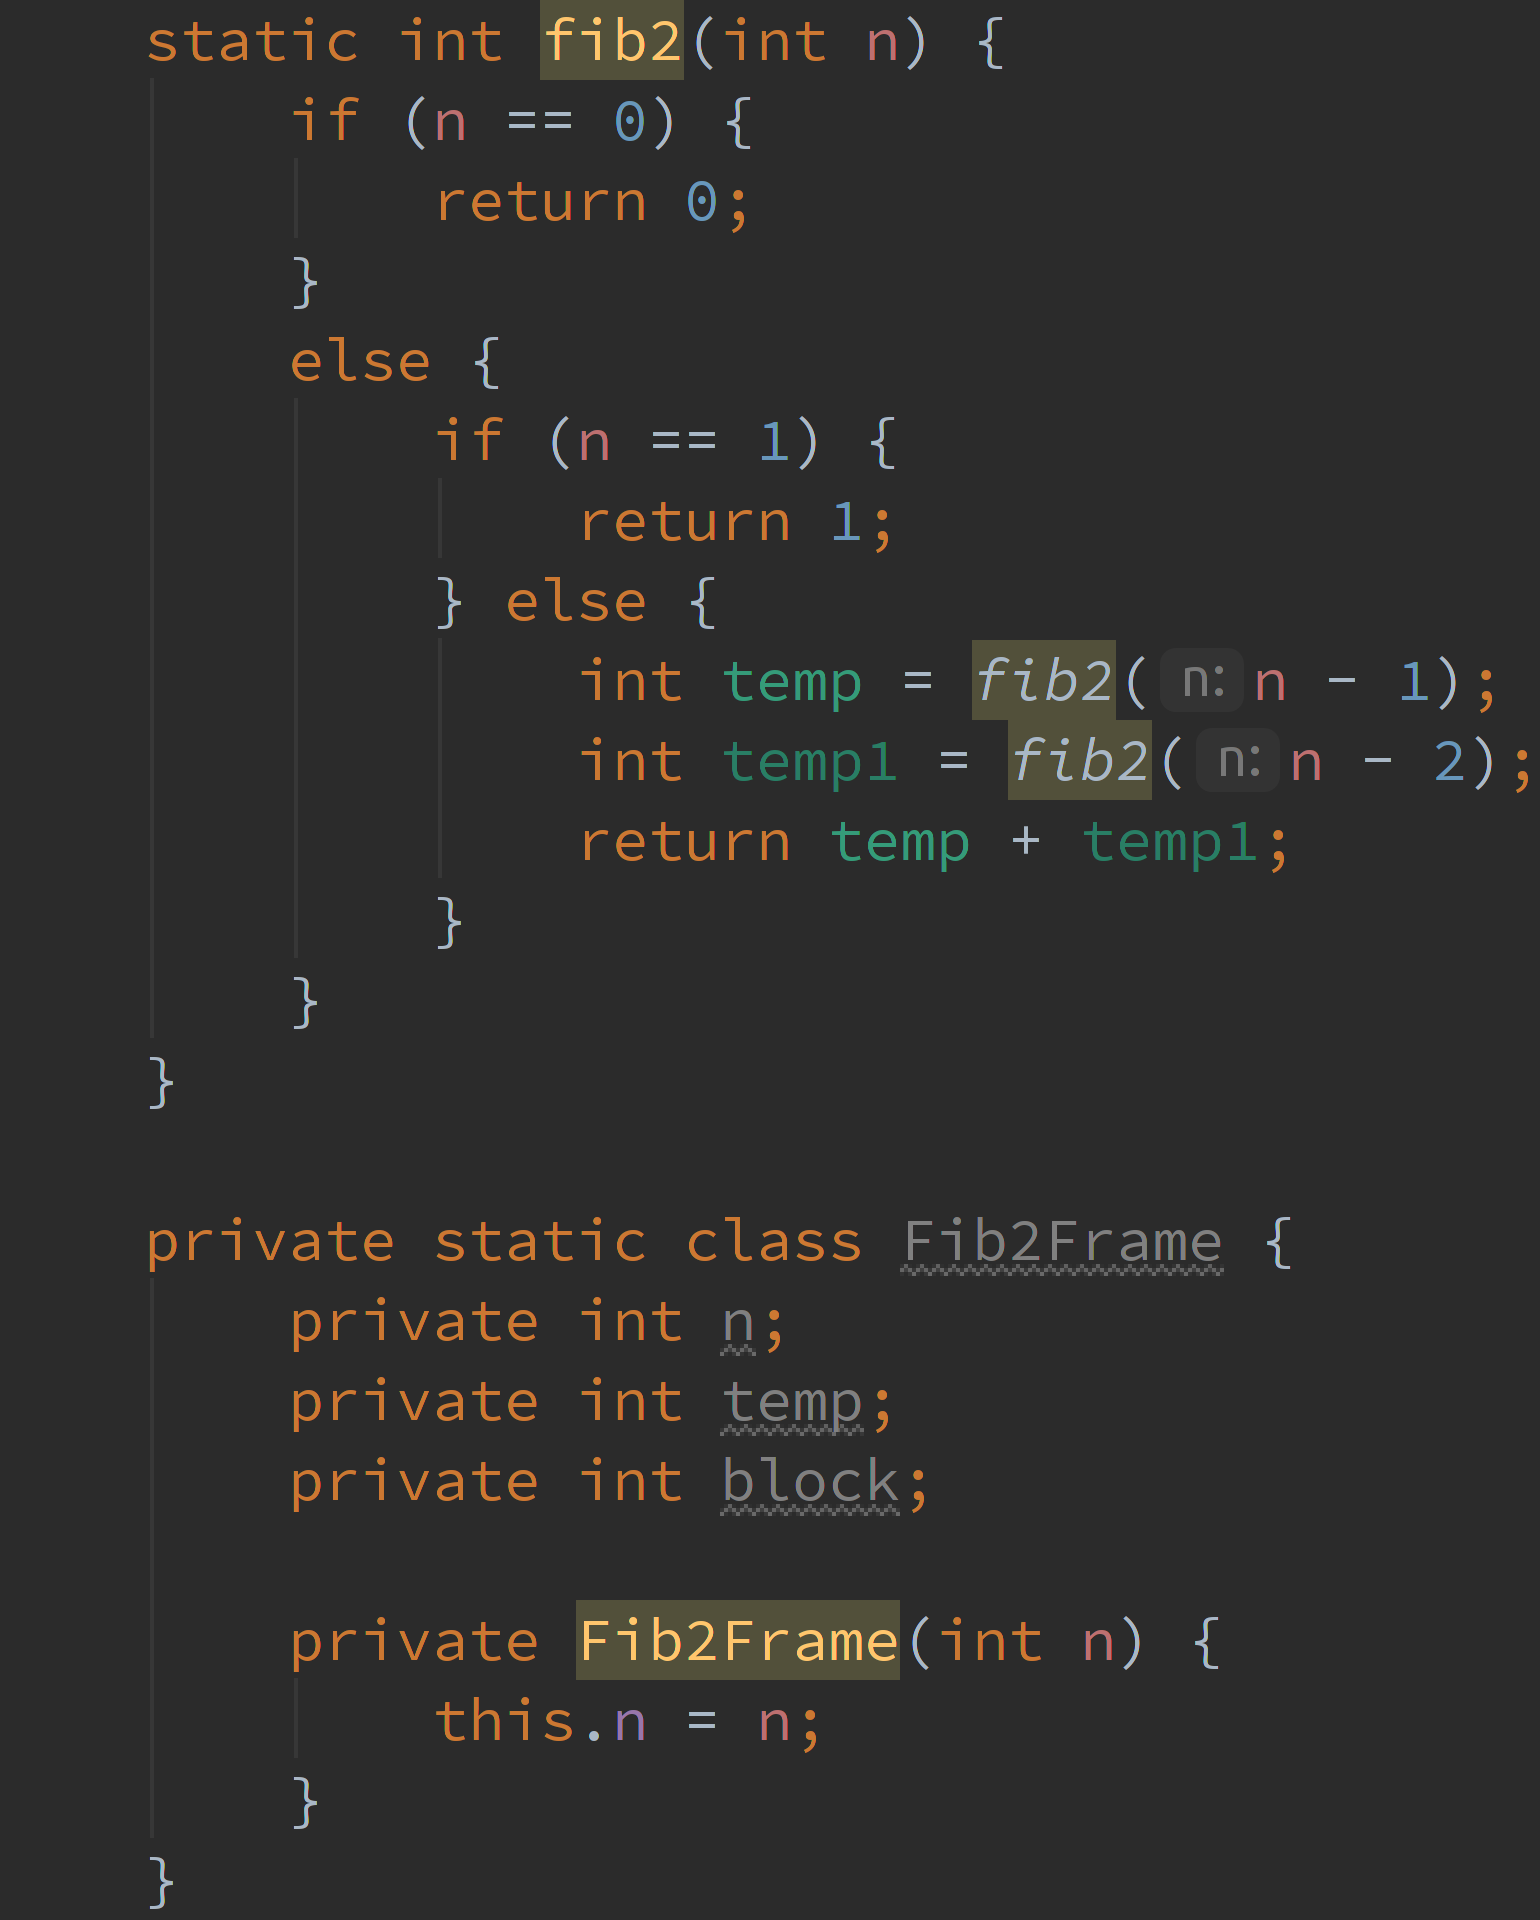
\includegraphics[height=2.5in]{src/img/incorporate-before.png}
        \caption{Before}
    \end{subfigure}%
    \begin{subfigure}[b]{.6\textwidth}
        \centering
        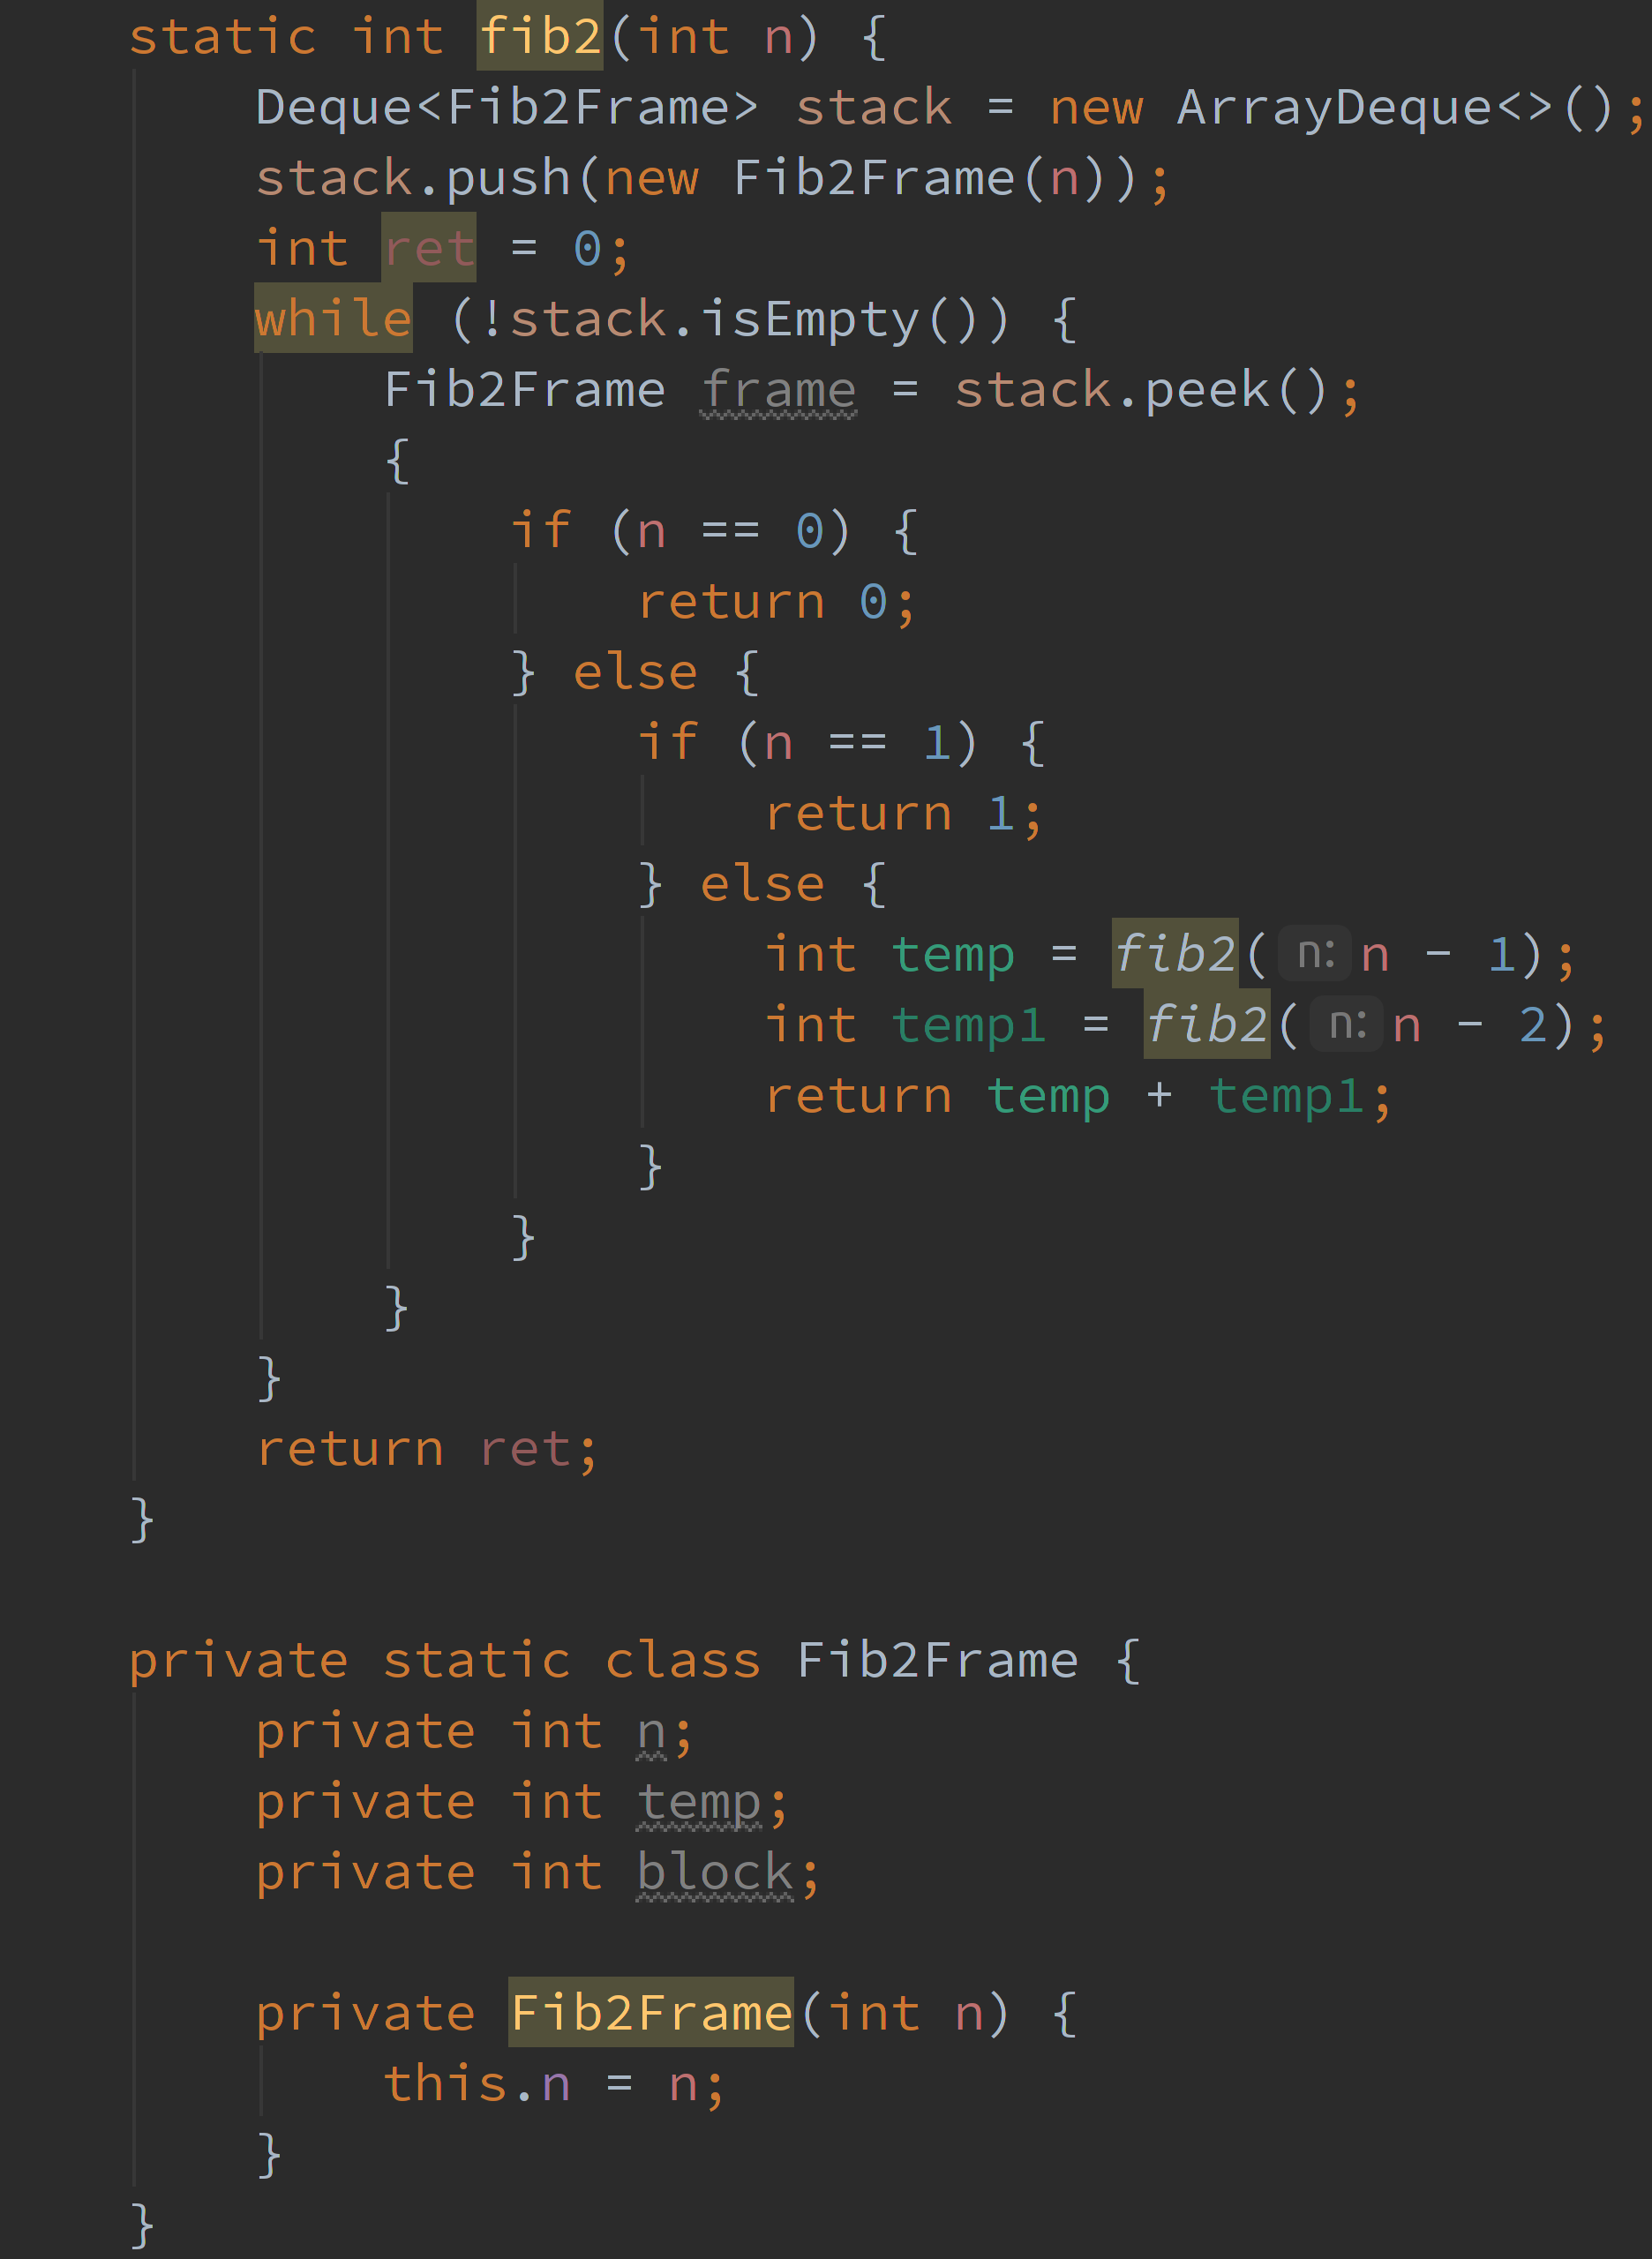
\includegraphics[height=3.33in]{src/img/incorporate-after.png}
        \caption{After}
    \end{subfigure}%
    }\\
    \caption{Incorporating the body \label{img:incorporate}}
\end{figure}